\documentclass[10pt,twocolumn,letterpaper]{article}

\usepackage{cvpr}
\usepackage{times}
\usepackage{epsfig}
\usepackage{graphicx}
\usepackage{amsmath}
\usepackage{amssymb}
\usepackage{multirow}
\usepackage{subfigure}
\usepackage[colorlinks,linkcolor=black,anchorcolor=blue,citecolor=red, urlcolor = blue, breaklinks=true,bookmarks=false]{hyperref} % Using hyper reference
\usepackage{indentfirst}
\usepackage{algpseudocode}
\usepackage[vlined,ruled,commentsnumbered]{algorithm2e}

\usepackage{hyperref}
\usepackage{url}
\usepackage{mwe}
\usepackage{float}
\usepackage{multirow}
\usepackage{indentfirst}
\usepackage{gensymb}
\usepackage{amssymb}
\usepackage{amsthm}
\usepackage{amsmath}
\usepackage{tabularx}
\usepackage{array}
\usepackage{diagbox}
\usepackage{array}
\usepackage{booktabs}
\usepackage[vlined,ruled,commentsnumbered]{algorithm2e}
\usepackage{algpseudocode}
\usepackage{amsmath}
\usepackage{graphicx}
\usepackage{subfigure}
\usepackage{epsfig}
\usepackage{verbatim}
\usepackage{wrapfig}
\usepackage{makecell}
\usepackage{indentfirst}


\cvprfinalcopy

\def\httilde{\mbox{\tt\raisebox{-.5ex}{\symbol{126}}}}

\begin{document}
\title{
  CS410 Artificial Intelligence\\
  Project Report
}

\author{
  ???\\
  \and
  ???\\
}

\maketitle

\begin{abstract}
Currently, the application of artificial intelligence (AI) is becoming more and more ubiquitous in our society and demonstrates its strength in many domains, such as image recognition, medical industry, natural language processing, gaming, self-driving cars and etc. Many of these applications are attibuted to data classification tasks such as sentiment analysis, image classification and medical diagnostics. Recent developments in neural network have greatly promoted the performance of data classification in those domains. In this work, we exploit a classification problem based on HG-U133A dataset\footnote{The dataset can be download from \url{https://www.ebi.ac.uk/arrayexpress/experiments/E-TABM-185/}} to conduct a thorough examination on both classical approaches (e.g. PCA, SVM) and deep learning methods. Besides, extensive comparative experiments with different configurations or hyper-parameters settings are carried out to demonstrate corresponding influence.
\footnote{Our code is avaiable at \url{https://github.com/shinshiner/Gene_Chip_Ananysis}}

\end{abstract}

\section{Introduction}

\label{sec:intro}
	A gene is a genomic sequence (DNA or RNA) which is the basic physical and functional unit of heredity. In humans, a gene can be directly functional or be the intermediate template for a protein that performs a specific function \cite{gene}. Most biological traits are under the influence of polygenes as well as gene-environment interactions \cite{whatisGene}. In particular, risk to a range of diseases is directly associated with corresponding genes or their mutation. Therefore, medical diagnostics to these diseases can be accomplished with gene analysis, which promises high accuracy \cite{globalViewOfGene, genegene}.
	
	In general, patients with same gene disease will also have common gene patterns in their chromosomes. Since the number of recognized gene diseases and the length of human gene sequence are actually limited \cite{geneLimit}, medical diagnostics to these diseases can be reduced to a classification problem, where given a sample of gene sequence, the output is a certain disease that matches the gene sequence. Theoretically, a huge database can be build to cover all possible human gene sequences with enough samples. However, since a human chromosome can have up to 500 million base pairs of DNA with thousands of genes, we are merely able to infer certain gene patterns from data analysis, and diagnose by deduction with current medical samples.
	
	Recently, the rapid developments in AI and gene probes have provided viable solutions on such classification problem \cite{MLinGene, geneProbe}, where each gene sample is represented with a high-dimensional feature vector given by the gene probe, and the problem thus becomes mathematical. There are two mainstream methods towards this problem: classical methods and deep learning.
	
	Classical methods tackling this problem are mainly related to dimension reduction and distance-based approaches. The dimension reduction is usually achieved with the \emph{principle component analysis} (PCA) algorithm \cite{pca}, where the original feature vector, consisting of a large set of feature values, is converted into a smaller set of values that are linearly uncorrelated called principal components. Distance-based methods include \emph{k-nearest neighbors} (k-NN) algorithm \cite{knn} that directly predicts results by comparing known data, and \emph{support vector machine} (SVM) \cite{svm} that classifies data with a reasonable loss function (e.g. \emph{Hinge loss} or \emph{cross-entropy loss}).
	
	Deep learning methods are based on interpretation of information processing and communication patterns in a biological nervous system, and attempt to model the classification problem with neural network architectures. Typical neural network uses a cascade of multiple layers of nonlinear processing units for feature extraction and transformation \cite{deepLearning1}. Each successive layer uses the output from the previous layer as input. With \emph{back propagation} \cite{BP}, the neural network can efficiently approximate the target function by doing \emph{gradient descent} with a \emph{loss function}.

	In this work, considering the high dimension of original feature vectors, we first do PCA to reduce the dimension. Then we apply both classical and deep learning methods to a multi-class classification problem based on \textit{HG-U133A} dataset. It turns out that both methods can achieve outstanding accuracy. In particular, our results show that deep learning method outperforms classical ones, especially in the aspect of the trade-off between efficiency and accuracy.

\section{Approaches}
\label{sec:approaches}
	We formulate the classification problem as followed: given $n$ samples $X = \{x_1, x_2, \dots, x_n\}$, where each $x_i$ is a $p$ dimension feature vector for the $i^{th}$ sample, and a set of labels $Y = \{y_1, y_2, \dots, y_n\}, y_i \in 1 \dots m$ from $m$ categories denoting that $x_i$ is classified into the $y_i^{th}$ category by ground truth. The task is to assign a single label to a feature vector from a fixed set of categories with knowledge from given samples.

	Our solution consists of two parts: \emph{dimension reduction} and \emph{classification}. We first apply PCA to achieve dimension reduction for the sake of accelerating computation. After that, we divide the dataset into training set and test set for \textit{cross validation} \cite{crossValidation}, and check the performance of different classification models on test set.
	
\subsection{Dimension Reduction}
	In given dataset, each sample is a 22283-dimension feature vector while the number of samples is merely $3558$ after preprocessing. This classification problem apparently belongs to large $p$ small $n$ problem, where $p$ is the dimension of feature vector and $n$ is the number of samples.
	
	On the basis of the above fact, PCA is necessary to tackle this problem. The process of PCA can be summarize as a linear mapping of feature vectors to a lower-dimensional space, where the linear correlation among variables are minimized.
	
	Consider $n$ feature vectors each of dimension $p$, whole PCA process is as follows:
\begin{enumerate}
\item Approximate the empirical mean vector $u$ from known samples by using the averaging expression
\begin{equation}
	u = \frac{1}{n} \sum_{i=1}^n x_i\label{eq:mean}
\end{equation}

\item Calculate the covariance matrix $C$ from the samples with
\begin{equation}
	C = \frac{1}{n-1} \sum_{i=1}^n x_i x_i^T - u u^T \label{eq:cx}
\end{equation}

\item Compute the eigenvectors and eigenvalues of the covariance matrix $C$, since $C$ is a symmetric matrix and thus can be diagonalized.
\begin{equation}
	V^T CV = D \label{eq:eig}
\end{equation}
	where the matrix $V$ consists of eigenvectors which diagonalizes the covariance matrix $C$, and $D$ is the diagonal matrix of eigenvalues of $C$.

\item Rearrange the eigenvectors and eigenvalues in a way that the columns of the eigenvector matrix $V$ and eigenvalue matrix $D$ are sorted in order of decreasing eigenvalue. The eigenvalues represent the distribution of the source data's energy among each of the eigenvectors, where the eigenvectors form a basis for the data.

\item Select the first $k$ columns of $V$ as the $p \times k$ matrix $W$, so that
\begin{equation}
	\frac{\sum_{i=1}^k D_{ii}}{\sum_{i=1}^p D_{ii}} \geq Thres \label{eq:dimR}
\end{equation}
	where $Thres$ is the desired proportion of cumulative energy. In our configuration, $Thres = 90\%$ and $k = 453$.

\item Project the z-scores of the data onto the new basis
\begin{equation}
	t_i = W^T (x_i - u)\label{eq:proj}
\end{equation}
\end{enumerate}
	
	After PCA, we successfully reduce the correlation of features, which considerably accelerates training in \textit{classification} stages. Moreover, the ''new'' feature vectors are centered (Eq. \eqref{eq:mean} \eqref{eq:proj}), which can be used for training without extra preprocessing.

\subsection{Classical Methods}
	The primary classical methods we use contain the \emph{k-nearest neighbors algorithm} and \emph{multi-class support vector machine}.

\subsubsection{K-nearest Neighbors Algorithm}
	k-NN is a non-parametric method used for pattern recognition and classification. Its idea is quite simple: given a sample $x$, the classifier will compute the distance between $x$ and other samples in dataset $X$. Then it will find the top $k$ closest samples $X^{'}$. In k-NN point of view, the most common class in $X^{'}$ will be the class of $x$. Intuitively, higher values of $k$ have a smoothing effect that makes the classifier more resistant to outliers. The pseudo code of k-NN can refer to Alg. \ref{alg:knn}.
	
\begin{algorithm}[htbp]
	\SetKwInOut{Input}{input}
	\SetKwInOut{Output}{output}
	\caption{K-nearest neighbors algorithm}\label{alg:knn}
	\vspace{0.25\baselineskip}
	\Input{Feature vector $u$, distance function $d(\cdot)$.}
	\Output{Classification label $v$ for $u$.}
	\BlankLine
	\For{$x \in X$}{
		Compute $d(x, u)$\;
	}
	Sort $x$ by $d(x, u)$ in increasing order\;
	$X' \leftarrow X_{1:k}$\;
	$v \leftarrow$ the most common label of feature vectors in $X'$\;
	\Return $v$;
\end{algorithm}
\BlankLine
	
	Note that the distance should be measured by a distance function. Although such function can be defined in many ways, the Euclidean metric is the most common practice which maps the straight-line distance between two points in Euclidean space. When comparing two feature vectors, one of the simplest possibilities is to compare the vectors element by element and add up all the differences. In other words, given two feature vectors $x_1, x_2$ with $p$ dimensions, a reasonable choice for comparing them might be the L1 distance:
\begin{equation}
	d_1(x_1, x_2) = \sum_p \left|x_1^p - x_2^p\right| \label{eq:l1}
\end{equation}

	Another common choice would be L2 distance, which has the geometric interpretation of computing the Euclidean distance between two vectors. The distance takes the form:
\begin{equation}
	d_1(x_1, x_2) = \sqrt{\sum_p {\left(x_1^p - x_2^p\right)}^2} \label{eq:l2}
\end{equation}
	
	From Alg. \ref{alg:knn}, it is obvious that k-NN is very simple to implement and understand. Besides, the classifier takes no need to train, since all it requires is to store and index the dataset. However, we pay quite a bit computational cost when testing, for each classification operation requires comparisons with all samples. This is one of its shortcomings, since in practice we often care about test efficiency more than training efficiency.
		
\subsubsection{Linear Classification}
	The linear classification approach has two major components: a \emph{score function} that maps the raw data to class scores, and a \emph{loss function} that quantifies the gap between the predicted scores and the ground truth labels. It can be cast as an optimization problem in which we attempt to minimize the loss function with respect to the parameters of the score function. \cite{svmCS231n}

\paragraph{Score Function}
	Basically, the score function of linear classification is a linear mapping
\begin{equation}
	f(x_i, W, b) = W x_i + b
\end{equation}
	where $x_i$ is the sample to be classified, the matrix $W$ (\emph{weights}, of size $[m \times p]$), and the vector $b$ (\emph{bias}, of size $[m \times 1]$) are the parameters of the function ($m$ and $p$ denote the number of classes and dimensions respectively).
	
	A significant advantage of this approach is that the training data is used to learn the parameters $W$ and $b$, once a satisfying $W, b$ is learned, we just need to keep the learned parameters. Then a new sample can be simply and efficiently forwarded through this function and classified based on the computed scores.

\paragraph{Loss Function}
	A \emph{loss function} (also called \textit{cost function} or \textit{objective}) aims to measure the incorrectness of classification. Intuitively, the loss will be high if the classifier does a poor job of classifying the samples, and it will be low if the classifier does well. There are several commonly used loss functions with different forms.

\paragraph{Hinge Loss (SVM)}
	In machine learning, a commonly used loss is the \emph{Multiclass Support Vector Machine} (SVM) loss, which is set up so that the SVM ``wants'' the correct class for each feature vector to have a score higher than the incorrect classes by some fixed margin $\Delta$.

	We use $s$ to represent the class scores returned by \textit{score function}. With the score for the $j^{th}$ class is the $j^{th}$ element: $s_j=f(x_i, W, b)_j$, the multiclass SVM loss for the $i^{th}$ sample is then formalized as followed:
\begin{equation}
	L_i = \sum_{j \neq y_i} max(0, s_j - s_{y_i} + \Delta)\label{eq:svmloss}
\end{equation}

	According to Eq. \eqref{eq:svmloss}, the SVM loss function wants the score of the correct class $y_i$ to be larger than the incorrect class scores by at least $\Delta$. If this is not the case, we will accumulate loss.
	
	Taking linear score functions ($f(x_i, W) = W x_i$) into consideration, the loss function can be rewritten in this equivalent form:
\begin{equation}
	L_i = \sum_{j \neq y_i} max(0, W_j^T x_i - W_{y_i}^T x_i + \Delta)
\end{equation}
	where $w_j$ is the $j^{th}$ row of $W$ reshaped as a column.
	
	With SVM loss function, the threshold at zero $max(0,-)$ function is often called the \emph{Hinge loss}. And the so-called \emph{squared hinge loss SVM} (or L2-SVM) uses the form $max(0,-)^2$ that penalizes violated margins more strongly. The unsquared version is more standard, but in some datasets the squared hinge loss can work better. This can be determined during cross-validation. \cite{svmCS231n}

\paragraph{Cross-entropy Loss (Softmax)}                             
	In addition to Hinge loss, Softmax classifier is also commonly used, which is the generalization of \emph{logistic regression} (LR) to multiple classes. Instead of treating the outputs $f(x_i, W)$ as scores for each class like SVM, Softmax classifier gives a more intuitive output (normalized class probabilities) and also has a probabilistic interpretation. 
	
	In Softmax classifier, the function mapping $f(x_i; W)=W x_i$ remains unchanged, but we now interpret these scores as the unnormalized log probabilities for each class and replace the Hinge loss with a cross-entropy loss that has the form:
\begin{equation}
	L_i = -\log \left( \frac{e^{f_{y_i}}}{\sum_{j} e^{y_j}}\right)
\end{equation}

	or equivalently
\begin{equation}
	L_i = -f_{y_i} + \log \sum_j e^{y_j}
\end{equation}
	where we are using the notation $f_j$ to represent the $j^{th}$ element of the vector of class scores. The function $f_j(z) = \frac{e^{f_{z_j}}}{\sum_{k} e^{z_k}}$ is called the \emph{softmax function}. It takes a vector of arbitrary real number scores and squashes it to a vector of values between 0 and 1, and the sum of them is 1. 

	The softmax function can be interpreted as the probability assigned to the correct label $y_i$ given the input $x_i$ and parameters $W$:
\begin{equation}
	P(y_i | x_i; W) = \frac{e^{f_{y_i}}}{\sum_{j} e^{y_j}}
\end{equation}

	In terms of information theory, the \emph{cross-entropy} between a ``true'' distribution $p$ and an estimated distribution $q$ is defined as
\begin{equation}
	H(p, q) = -\sum p(x) \log q(x)
\end{equation}

	Softmax classifier is hence minimizing the cross-entropy between the estimated class probabilities and the ``true'' distribution, which in this interpretation is the distribution where all probability mass is on the correct class (i.e. $p=[0,\dots 1,\dots, 0]$ contains a single 1 at the $y_i^{th}$ position). Moreover, since the cross-entropy can be written in terms of entropy and the Kullback-Leibler divergence \cite{KLdivergence} as 
\begin{equation}
	H(p, q) = H(p) + D_{KL}(p||q)
\end{equation}
	and the entropy of the delta function $p$ is 0, this is also equivalent to minimizing the KL divergence between the two distributions (a measure of distance). In other words, the cross-entropy loss function wants the predicted distribution to have all of its mass on the correct answer.

\paragraph{Regularization}
	It seems that the loss functions above make sense. Nevertheless, these functions do have a defect. Suppose that we have a dataset and a set of parameters $W$ that correctly classify all samples (i.e. all scores are so perfect that all the margins are met, and $L_i=0$ for any sample $x_{i}$). The issue is that this $W$ is not necessarily unique: there might be many similar $W$ that correctly classify the samples. One easy way to see this is that if some parameters $W$ correctly classify all samples (so loss is 0 for each sample), then any multiple of these parameters $\lambda W$ where $\lambda > 1$ will also give 0 loss because this transformation uniformly stretches all score magnitudes and hence also their absolute differences. \cite{svmCS231n}
	
	Basically, we want to encode some preference for a certain set of weights $W$ over others to remove this ambiguity. We can achieve this by extending the loss function with a regularization penalty $R(W)$ item. The most common regularization penalty is the L2 norm that discourages large weights through an elementwise quadratic penalty over all parameters:
\begin{equation}
	R(W) = \sum_{k} \sum_{l} W_{k, l}^2
\end{equation}

	Similarly, the L1 norm is formulated as 
\begin{equation}
	R(W) = \sum_{k} \sum_{l} \left|W_{k, l}\right|
\end{equation}

	With regularization penalty involved, the loss function becomes complete and more robust, which consists of two components: the data loss (which is the average loss of all samples) and the regularization loss. Therefore, using $N$ to denote the number of training samples, the full loss function becomes:
\begin{equation}
	L = \frac{1}{N} \sum_i L_i + \lambda R(W)
\end{equation}
	
	Generally speaking, such penalty for large weights tends to improve generalization ability and avoid overfitting problem, because it means that no input dimension can have a very large influence on the scores. However, in practice, the parameters might be hard to converge due to the regularization penalty, we can never achieve loss of exactly 0 for all samples, because this would only be possible in the pathological setting of $W=0$.

\subsubsection{Deep Learning}
	The concept of Neural Networks (NN) is originally inspired by the goal of modeling biological neural systems, but has since diverged and become a matter of engineering and achieving good results in Machine Learning tasks.

\paragraph{The Neuron Model}
	The basic computational unit of the brain is a neuron. As is shown in Fig. \ref{fig:neurons}, each neuron receives input signals from its \emph{dendrites} and produces output signals along its \emph{axon}. The axon eventually branches out and connects via synapses to dendrites of other neurons. In the computational model of a neuron, the signals that travel along the axons (e.g. $x_0$) interact multiplicatively (e.g. $w_0 x_0$) with the dendrites of the other neuron based on the synaptic strength at that synapse (e.g. $w_0$). The idea is that the synaptic strengths (the weights $w$) are learnable and control the strength of influence (and its direction: excitory (positive weight) or inhibitory (negative weight)) of one neuron on another. In the basic model, the dendrites carry the signal to the cell body where they all get summed. If the final sum is above a certain threshold, the neuron can fire, sending a spike along its axon. In the computational model, we assume that the precise timings of the spikes do not matter, and that only the frequency of the firing communicates information. Based on this rate code interpretation, we model the firing rate of the neuron with an activation function $f$, which represents the frequency of the spikes along the axon. \cite{neuronModel}

\begin{figure}[htbp]
	\centering
	\subfigure[A biological neuron]{
	    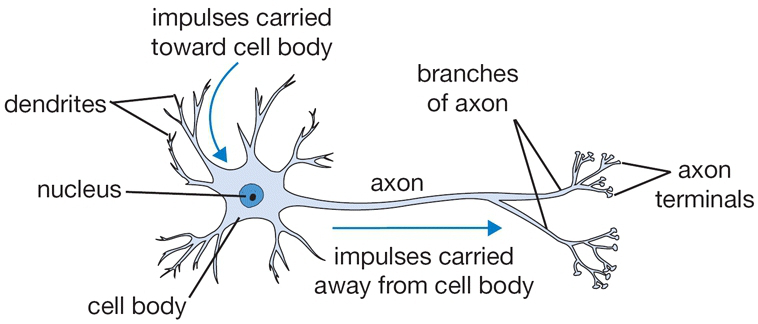
\includegraphics[width=0.9\linewidth]{images/neuron.png}
	}

	\subfigure[A common mathematical model]{
	    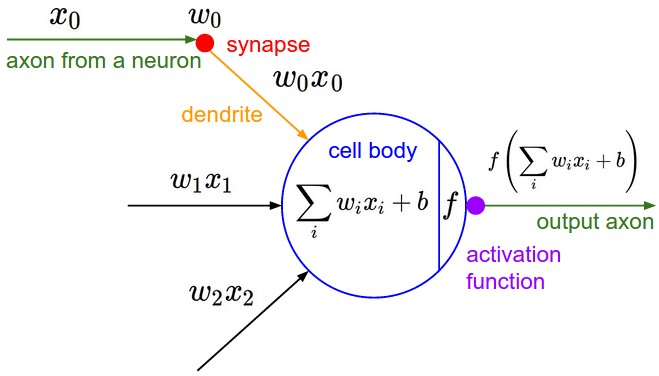
\includegraphics[width=0.9\linewidth]{images/neuron_model.jpeg}
	}
	\caption{Biological motivation of the neuron model. \cite{neuronModel}}
	\label{fig:neurons}
\end{figure}

\paragraph{Activation Function}
	Every activation function (or non-linearity) takes a single number as input and performs a certain fixed mathematical operation on it. There are several activation functions that are commonly used.
\begin{itemize}
\item \textbf{Sigmoid} The mathematical form of sigmoid non-linearity is as followed.
\begin{equation}
	\sigma(x) = \frac{1}{1 + e^{-x}}
\end{equation}
	It takes a real number and ``squashes'' it into range between $0$ and $1$. In particular, large negative numbers become $0$ and large positive numbers become $1$. The sigmoid function has been frequent used historically since it has a nice interpretation as the firing rate of a neuron. 

\item \textbf{Tanh} The tanh non-linearity squashes a real number to the range $[-1, 1]$. 
\begin{equation}
	tanh(x) = x \sigma (2x) - 1
\end{equation}

	Like sigmoid activation function, its activations saturate, but its output is zero-centered. Therefore, the tanh non-linearity is always preferred to the sigmoid nonlinearity in practice.

\item \textbf{ReLU}\cite{relu} The full name of ReLU is \textit{Rectified Linear Unit}, which has become very popular in the last few years. It computes the function 
\begin{equation}
	f(x) = max(0, x)
\end{equation}
	It was found to greatly accelerate the convergence of stochastic gradient descent (SGD) compared to the sigmoid or tanh functions due to its linear, non-saturating form. However, ReLU units can be fragile during training and might never activate on some neurons faced with a large gradient flowing.
\end{itemize}

\paragraph{Neural Network Architectures}
	Neural networks are modeled as collections of neurons that are connected in an acyclic graph. In other words, the outputs of some neurons can become inputs to other neurons. Neural network models are often organized into distinct layers of neurons. For regular neural networks, the most common layer type is the fully-connected layer in which neurons between two adjacent layers are fully pairwise connected, but neurons within a single layer share no connections. 
	
	One way to look at Neural Networks with fully-connected layers is that they define a family of functions that are parameterized by the weights of the network. It has been proved that neural networks with at least one hidden layer are universal approximators that can approximate any continuous function \cite{sigmoid}. And deeper networks (with multiple hidden layers) can work better than a single-hidden-layer networks is an empirical observation, despite the fact that their representational power is equal.

\paragraph{Weight Initialization}
	Before we can begin to train the network we have to initialize its parameters. To avoid all-zero initialization, we want the weights to be very close to zero, but not identically zero. Also, an initialized neuron shouldn't have a variance that grows with the number of inputs. It turns out that we can normalize the variance of each neuron's output to 1 by scaling its weight vector by the square root of its fan-in (i.e. its number of inputs). That is, the recommended heuristic is to initialize each neuron's weight vector as:
\begin{equation}
	w \sim N\left(0, \frac{1}{\sqrt{n}}\right)
\end{equation}
	where $n$ is the number of its inputs. This ensures that all neurons in the network initially have approximately the same output distribution and empirically improves the rate of convergence. \cite{weightInit}

\paragraph{Regularization}
	There are several ways of controlling the capacity of Neural Networks to prevent overfitting \cite{svmCS231n}:
\begin{itemize}
\item \textbf{L2 Regularization} is perhaps the most common form of regularization. It can be implemented by penalizing the squared magnitude of all parameters directly in the objective. That is, for every weight $w$ in the network, we add the term $\frac{1}{2}\lambda w^2$ to the objective, where $\lambda$ is the regularization strength. It is common to see the factor of $\frac{1}{2}$ in front because then the gradient of this term with respect to the parameter $w$ is simply $\lambda w$ instead of $2\lambda w$.

\item \textbf{L1 Regularization} is another relatively common form of regularization, where for each weight $w$ we add the term $\lambda \left| w \right|$ to the objective. It is possible to combine the L1 regularization with the L2 regularization: $\lambda_1 \left| w \right| + \lambda_2 w^2$ \cite{Zou2005Zou}. The L1 regularization has the intriguing property that it leads the weight vectors to become sparse during optimization (i.e. very close to exactly zero). In other words, neurons with L1 regularization end up using only a sparse subset of their most important inputs and become nearly invariant to the ``noisy'' inputs. In comparison, final weight vectors from L2 regularization are usually diffuse, small numbers.

\item \textbf{Dropout} is an extremely effective, simple and recently introduced regularization technique. Dropout is implemented by only keeping a neuron active with some probability $p$ (a hyperparameter), or setting it to 0 otherwise during training time.
\end{itemize}

\paragraph{Loss Functions}
	The loss functions commonly used in deep learning are identical to those used in linear classifiers, including \emph{the SVM loss function}, \emph{cross-entropy loss function} and the \emph{$p$-norm loss} of form:
\begin{equation}
	L_i = {\left[ \sum_j {\left( f - y_j \right)}^n \right]}^{\frac{1}{i}}
\end{equation}
	
	For the multi-class classification task, it is common to compute the loss between the predicted quantity and the true answer and then measure the L2 squared norm, or L1 norm of the difference.


\section{Experiments and Results}
In this section, the model settings and results of our experiments will be introduced in detail.

\subsection{Preprocess}

Among all labels in \textit{E-TABM-185.sdrf.txt}, we choose the \textit{DiseaseState} item as classification target. However, there are some samples lack this label and some disease states rarely appear, we remove those samples which have no disease state label or corresponding labels appear less than 10 times. Additionally, we merge those samples with same disease and different stages into one label.

Ultimately, we extract 3558 samples, labeled with 76 classes. Then we divide the dataset into \emph{training set} and \emph{test set} with a ratio of 9:1 for each class in perparation for further cross validation. After the division, the  size of the datasets are shown in Table \ref{tab:crossV}.

\begin{table}[H]
	\centering
	\caption{Size of the trainset and test set}
	\label{tab:crossV}
	\begin{tabular}{lcc}
		\specialrule{0em}{1pt}{1pt}	
		\hline
		\specialrule{0em}{1pt}{1pt}
		Dataset & Training set & Test set \\
		\hline
		\hline
		\specialrule{0em}{1pt}{1pt}
		Size & 3203 & 355 \\
		\specialrule{0em}{1pt}{1pt}
		Ratio & 90\% & 10\% \\
		\hline
	\end{tabular}
\end{table}

\subsection{Principal Components Analysis}
	The PCA approach is applied for dimension reduction. According to Eqs. \eqref{eq:mean} \eqref{eq:cx} \eqref{eq:eig} \eqref{eq:dimR} \eqref{eq:proj}, we can compute the eigenvectors and eigenvalues of the covariance matrix, and represent the feature vectors with lower dimensions. Fig. \ref{fig:pca} and Table \ref{tab:pca} shows some of the intermediate results of PCA. 

\begin{figure}[H]
	\centering
	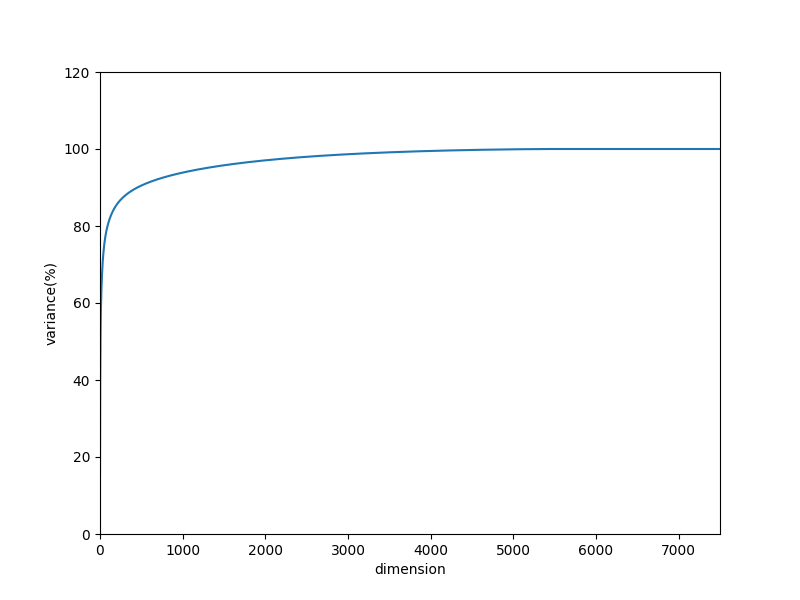
\includegraphics[width=0.97\linewidth]{images/pca.png}
	\caption{The accumulated percentage-dimension curve.}
	\label{fig:pca}
\end{figure}

\begin{table}[H]
	\centering
	\caption{Dimensions required by different variance percentages}
	\label{tab:pca}
	\begin{tabular}{ll}
		\specialrule{0em}{1pt}{1pt}	
		\hline
		\specialrule{0em}{1pt}{1pt}
		Variance percentage & Dimensions \\
		\hline
		\hline
		\specialrule{0em}{1pt}{1pt}
		15.23\% & 1 \\
		\specialrule{0em}{1pt}{1pt}
		49.89\% & 7 \\
		\specialrule{0em}{1pt}{1pt}
		85\% & 187 (0.84\%) \\
		\specialrule{0em}{1pt}{1pt}
		90\% & 453 (2.03\%) \\
		\specialrule{0em}{1pt}{1pt}
		95\% & 1271 (5.70\%) \\
		\hline
	\end{tabular}
\end{table}

	To preserve 90\% of the original variance, we reduce the original 22283 dimensions into 453 new dimensions, which accounts for roughly 2.03\% of the original number of dimensions. 

\subsection{K-Nearest Neighbors}
	In the experiments, we applied the k-NN algorithm with different parameter $k$ and various distance functions. 

\begin{table}[H]
	\centering
	\caption{Performances of k-NN with different parameters}
	\label{tab:knn}
	\begin{tabular}{lccc}
		\specialrule{0em}{1pt}{1pt}	
		\hline
		\specialrule{0em}{1pt}{1pt}
		L1 distance & $k=1$ & $k=3$ & $k=5$ \\
		\hline
		\hline
		\specialrule{0em}{1pt}{1pt}
		Accuracy & 83.792\% & 85.627\% & 85.627\% \\
		\specialrule{0em}{1pt}{1pt}
		F1-score & 83.531\% & 84.662\% & 84.700\% \\
		\hline
		\specialrule{0em}{3pt}{3pt}	
		\hline
		\specialrule{0em}{1pt}{1pt}
		L2 distance & $k=1$ & $k=3$ & $k=5$ \\
		\hline
		\hline
		\specialrule{0em}{1pt}{1pt}
		Accuracy & 85.321\% & 85.915\% & 84.098\% \\
		\specialrule{0em}{1pt}{1pt}
		F1-score & 85.200\% & 84.104\% & 83.679\% \\
		\hline
	\end{tabular}
\end{table}

	As is shown in Table \ref{tab:knn}, the accuracy and F1-score achieved by k-NN with various parameter settings are similar. In general, a larger $k$ performs better with  L1 distance, while a smaller $k$ can achieve high accuracy when L2 distance is used.

\subsection{Linear classifier}
	In this part of experiment, we try configurations with different learning rates,  regularization strengths and loss functions to determine the best configuration corresponding to each loss function. In all experiments, L2 regularization and the \emph{Adam} \cite{adam} optimizer is used to do gradient descent. The satisfactory results are shown in Table \ref{tab:lc}.
\begin{table}[H]
	\centering
	\caption{Performances of linear classifier with different loss functions}
	\label{tab:lc}
	\begin{tabular}{lcc}
		\specialrule{0em}{1pt}{1pt}	
		\hline
		\specialrule{0em}{1pt}{1pt}
		Loss function & SVM loss & Softmax loss \\
		\hline
		\hline
		\specialrule{0em}{1pt}{1pt}
		Learning rate & $5 \times 10^{-5}$ & $5 \times 10^{-5}$ \\
		\specialrule{0em}{1pt}{1pt}
		$\lambda$ & $1$ & $0.1$ \\
		\specialrule{0em}{1pt}{1pt}
		Accuracy & $88.45$\% & $89.86$\% \\
		\specialrule{0em}{1pt}{1pt}
		Epochs & 17 & 9 \\
		\hline
	\end{tabular}
\end{table}

	We also record the learning process of our linear classifers, the corresponding curves can refer to Fig. \ref{fig:lc_svm} \ref{fig:lc_softmax}.
\begin{figure}[htbp]
	\centering
	\subfigure[Training Accuracy]{
	    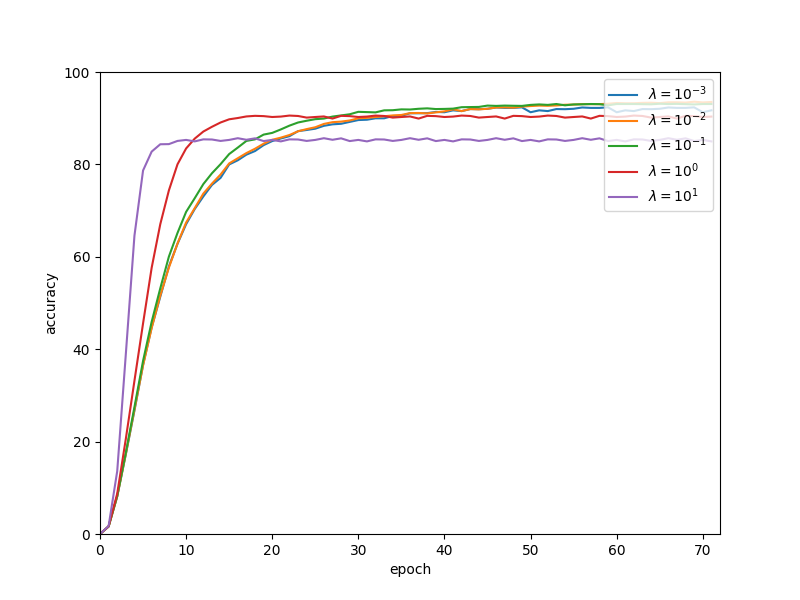
\includegraphics[width=0.474\linewidth]{images/lc_svm_train.png}
	}
	\subfigure[Test Accuracy]{
		    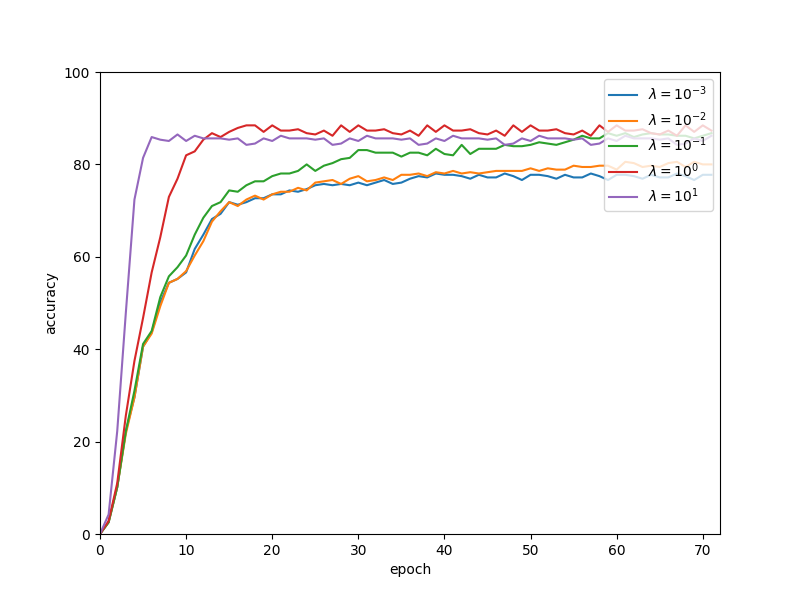
\includegraphics[width=0.474\linewidth]{images/lc_svm_test.png}
		}
	\subfigure[Loss]{
	    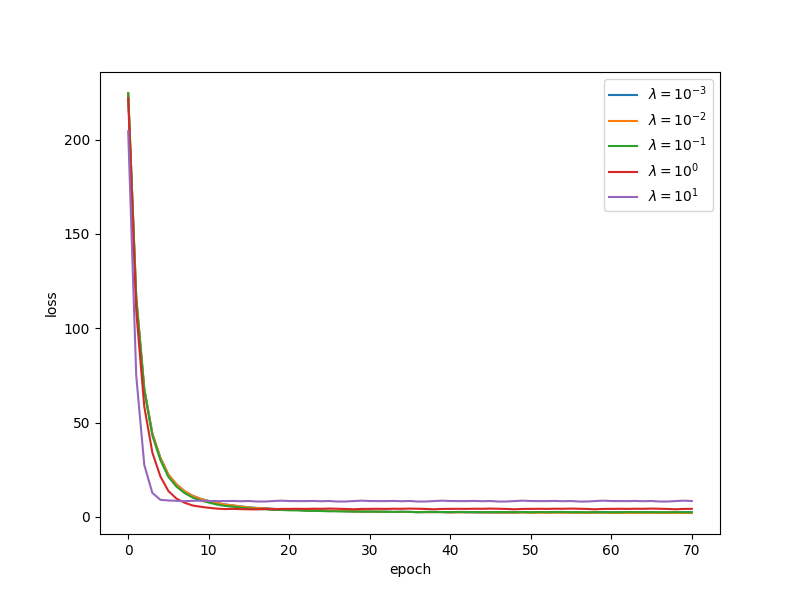
\includegraphics[width=0.5\linewidth]{images/lc_svm_loss.png}
	}
	\caption{Learning curves of linear classifier with SVM loss.}
	\label{fig:lc_svm}
\end{figure}
\begin{figure}[htbp]
	\centering
	\subfigure[Training Accuracy]{
	    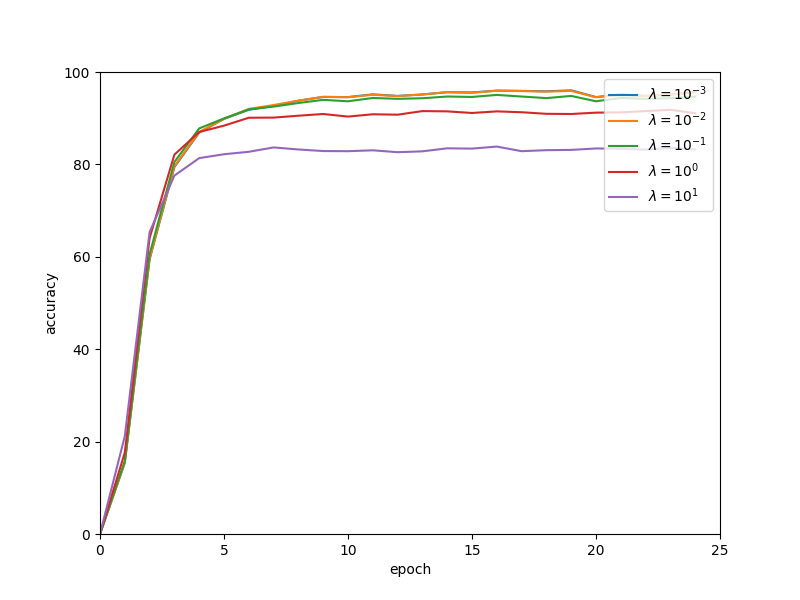
\includegraphics[width=0.474\linewidth]{images/lc_softmax_train.png}
	}
	\subfigure[Test Accuracy]{
		    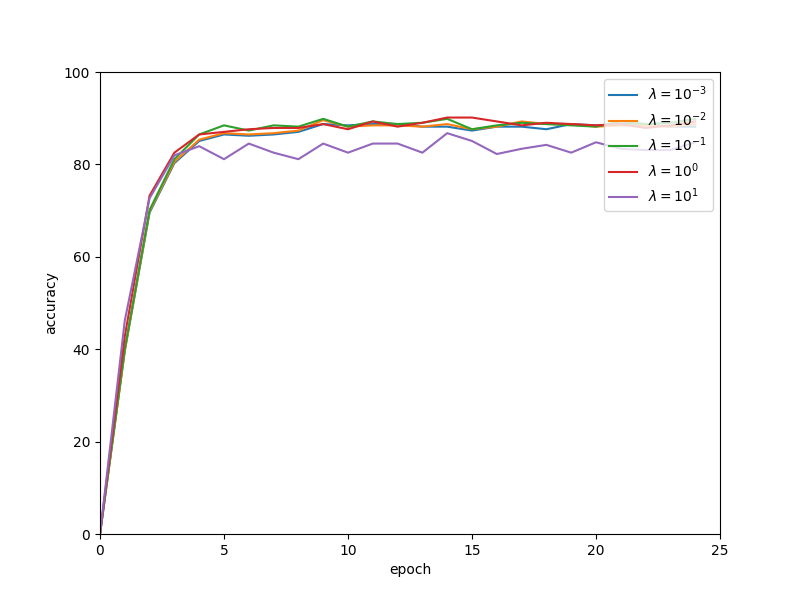
\includegraphics[width=0.474\linewidth]{images/lc_softmax_test.png}
		}
	\subfigure[Loss]{
	    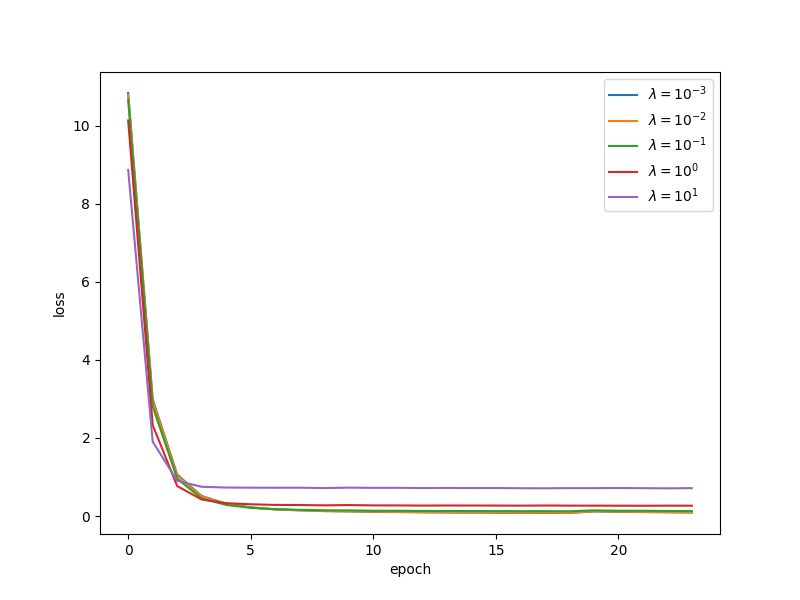
\includegraphics[width=0.5\linewidth]{images/lc_softmax_loss.png}
	}
	\caption{Learning curves of linear classifier with Softmax loss.}
	\label{fig:lc_softmax}
\end{figure}

\subsection{Deep learning}
	Our neural network model consists of 4 layers, each layer is regularized with L2 norm and activated by ReLU function. 50\% dropout \cite{dropout} is involved in hidden layers aiming to avoid overfitting. We start with learning rate of $5 \times 10^{-5}$ and train the model with the \emph{Adam} optimizer. Our network architecture can refer to Fig \ref{fig:net_architecture}. Still, we compare the results achieved with 2 different loss functions: SVM and Softmax in Table \ref{tab:dl}.
	
\begin{figure}[htbp]
	\centering
	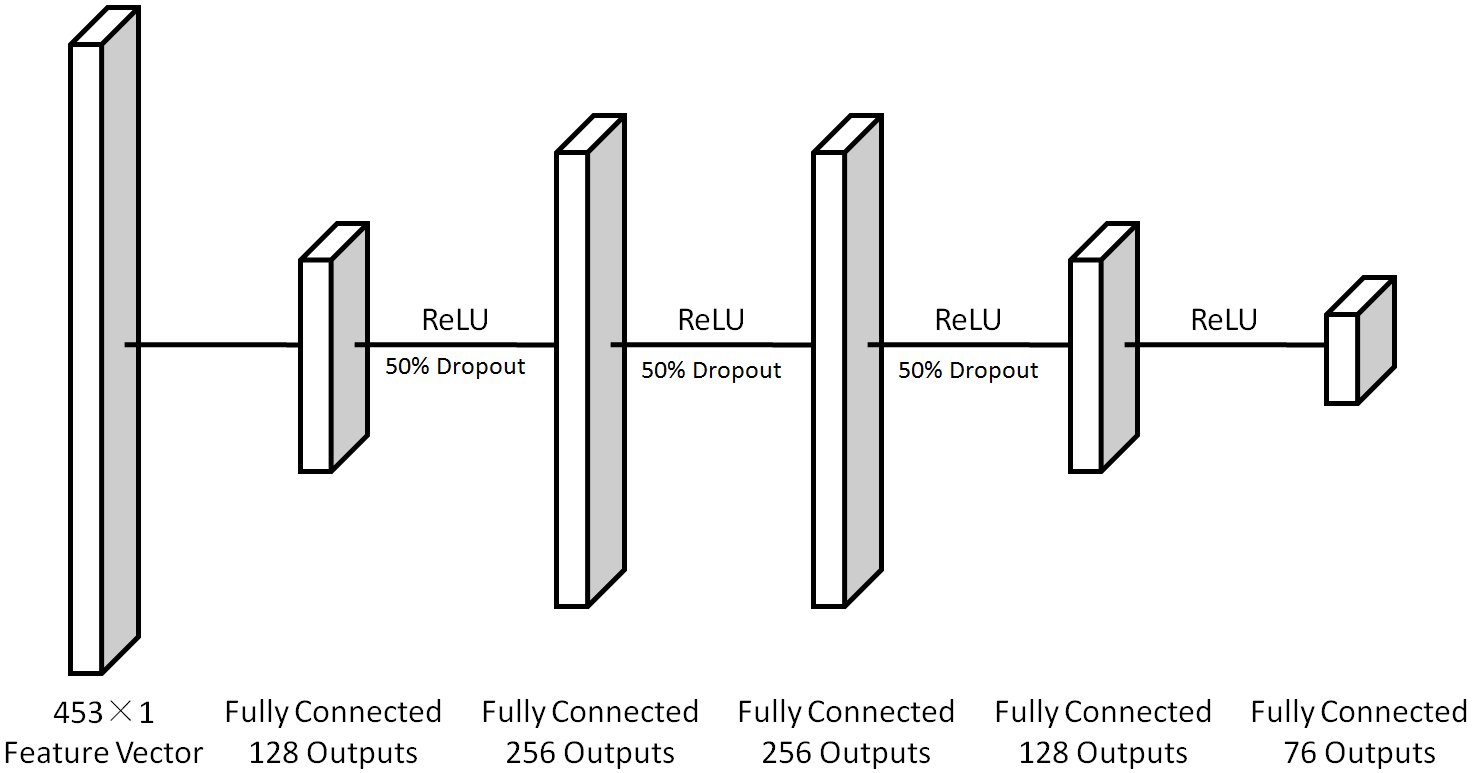
\includegraphics[width=0.95\linewidth]{images/network_architecture.png}
	\caption{Network Architecture.}
	\label{fig:net_architecture}
\end{figure}

\begin{table}[H]
	\centering
	\caption{Performances of neural network with different loss functions}
	\label{tab:dl}
	\begin{tabular}{lcc}
		\specialrule{0em}{1pt}{1pt}	
		\hline
		\specialrule{0em}{1pt}{1pt}
		Loss function & SVM loss & Softmax loss \\
		\hline
		\hline
		\specialrule{0em}{1pt}{1pt}
		$\lambda$ & $10^{-6}$ & $10^{-4}$ \\
		\specialrule{0em}{1pt}{1pt}
		Accuracy & 88.24\% & 91.27\% \\
		\specialrule{0em}{1pt}{1pt}
		Epochs & 12 & 18 \\
		\hline
	\end{tabular}
\end{table}

	The learning curves of neural network are shown in Fig. \ref{fig:dl_svm} \ref{fig:dl_softmax}.
\begin{figure}[htbp]
	\centering
	\subfigure[Training Accuracy]{
	    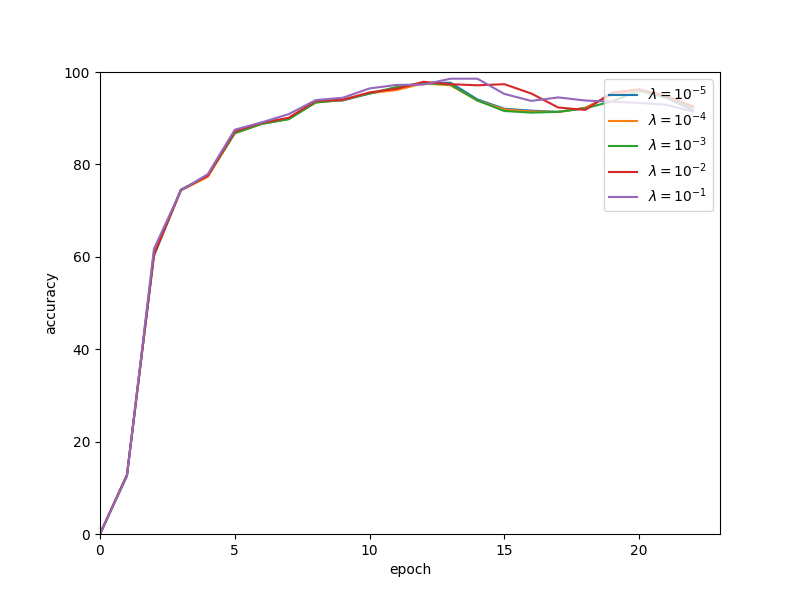
\includegraphics[width=0.474\linewidth]{images/nn_svm_train.png}
	}
	\subfigure[Test Accuracy]{
		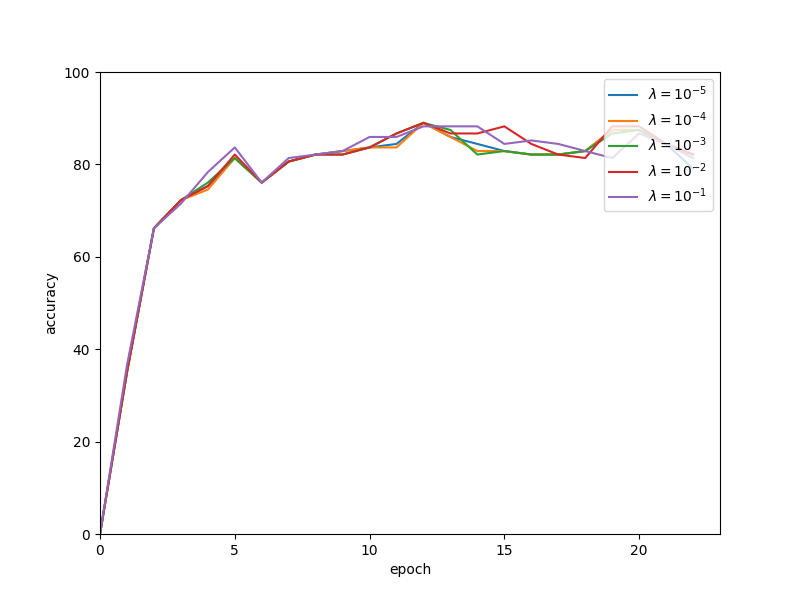
\includegraphics[width=0.474\linewidth]{images/nn_svm_test.png}
		}
	\subfigure[Loss]{
	    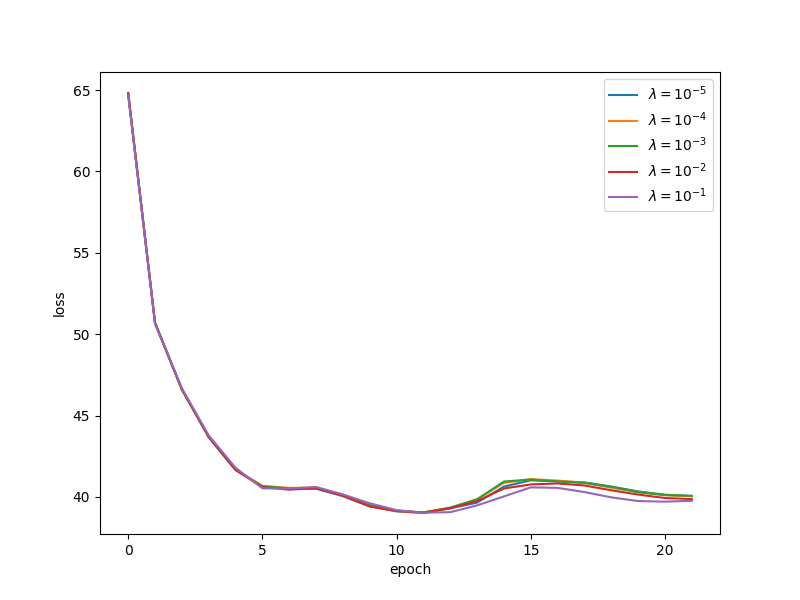
\includegraphics[width=0.5\linewidth]{images/nn_svm_loss.png}
	}
	\caption{Learning curves of neural network with SVM loss.}
	\label{fig:dl_svm}
\end{figure}
\begin{figure}[htbp]
	\centering
	\subfigure[Training Accuracy]{
	    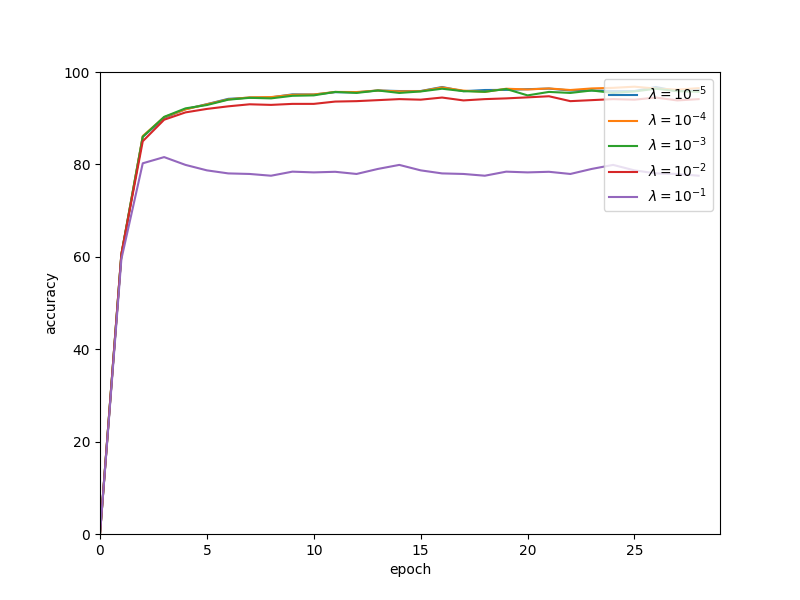
\includegraphics[width=0.474\linewidth]{images/nn_softmax_train.png}
	}
	\subfigure[Test Accuracy]{
		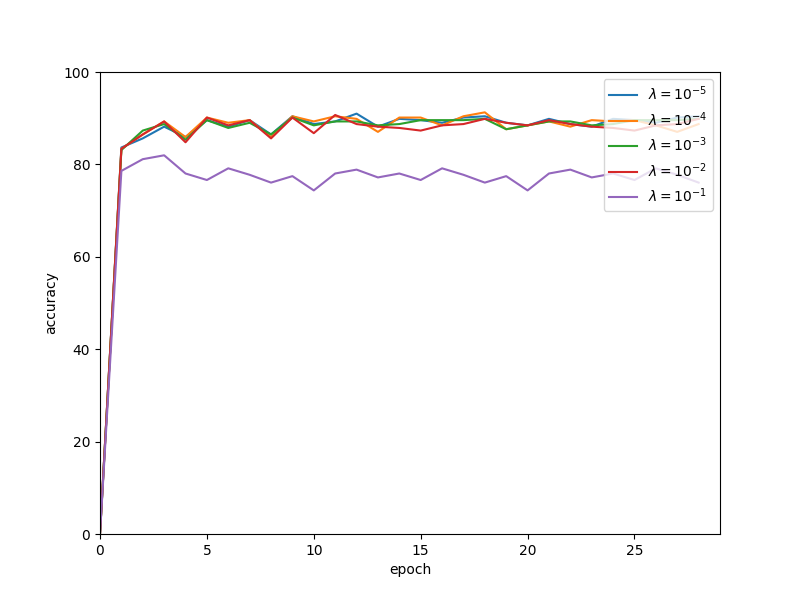
\includegraphics[width=0.474\linewidth]{images/nn_softmax_test.png}
	}
	\subfigure[Loss]{
	    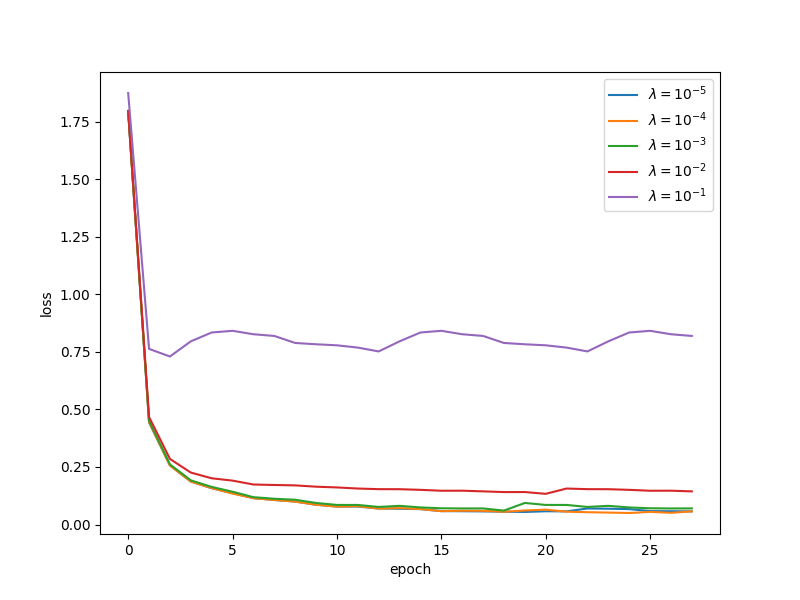
\includegraphics[width=0.5\linewidth]{images/nn_softmax_loss.png}
	}
	\caption{Learning curves of neural network with Softmax loss.}
	\label{fig:dl_softmax}
\end{figure}

\section{Discussion}

	\paragraph{PCA Parameter Choosing} For dimension reduction, PCA proves to be a powerful and reliable method, which contributes to a trade-off between data precision and computation cost. In general, several largest eigenvalues are large enough to cover more than half of total variance, and it takes more dimensions to preserve and more percent of variance as the precision increases. Therefore, we select 90\% as the threshold of preserved variance by experience to dramatically reduce the dimensions while preserving enough precision at the same time. Further investigation can be done by comparing training results based on cross-validation with different PCA projections to decide the best threshold.
	
	\paragraph{K-NN Parameter Choosing} Different hyper-parameter $k$ and distance function would result in slight, but not negligible impacts on classification performance. According to our experiments, a larger $k$ would achieve better results as noises have a smaller influence on it. However, an overlarge $k$ might also cause \emph{overfitting} which affects its performance. There are also differences between the two distance metrics (L1 and L2). In particular, the L2 distance is much more unforgiving than the L1 distance when it comes to differences between two vectors. That is, the L2 distance prefers many medium disagreements to one big one.
	
	\paragraph{Deep Learning Parameter Choosing} Considering the complexity of deep learning model, it is significant to avoid overfitting or local minimum. Thus, the choosing of learning rate and regularization coefficient $\lambda$ does matter. Actually, fixed learning rate can not generate high quality model for the lack of flexibility, it would be better to decrease it gradually instead in practice. As for regularization coefficient, generally speaking, high $\lambda$ can reduce variance and avoid overfitting, but extra bias would be involved, while low $\lambda$ can reduce bias but suffer from overfitting problem. The trade-off between variance and bias is hence critical.
	
	\paragraph{Loss Functions Selection} It turns out that the selection of loss functions is critical to final results. Basically, loss functions consists of data loss and regularization loss, and the trade-off between them is adjusted by $\Delta$ and $\lambda$.
	
	Within data loss, compared with SVM loss (Hinge loss), Softmax loss function proves more stable faced with large numbers as the normalization step prevents the gradient to explode. Actually, the performance difference between the SVM and Softmax are usually very small, and different people will have different opinions on which classifier works better.
	
	Compared to the Softmax classifier, the SVM is a more local objective, which could be thought of either as a bug or a feature. In other words, the Softmax classifier is never fully happy with the scores it produces: the correct class could always have a higher probability and the incorrect classes always a lower probability and the loss would always get better. However, the SVM is happy once the margins are satisfied and it does not micromanage the exact scores beyond this constraint.
	
	\paragraph{Linear Classifer \& Kernel-based Classifer}
	According to the results of our k-NN experiments, we can consider that the given dataset is linear separatable. Linear classifer is hence a more appropriate method under this circumstance.
	
	\paragraph{Classical Methods \& Deep Learning} The major advantage of neural network compared with linear classifiers, lies in its non-linear activation function, which enables it to approximate any continuous function. Therefore the representation power of deep neural network is stronger that linear models, and this power increases with the network depth. In addition, neural networks work well in practice because they compactly express nice, smooth functions that fit well with the statistical properties of data we encounter in practice, and are also easy to learn using our optimization algorithms (e.g. gradient descent).


\section{Conclusion and Thinking}
	In this project, we apply the classical classification methods and deep learning method to implement classification of diseases based on gene chip information and achieve satisfactory results. However, I think deep learning in this problem has not shown its real strength. Acturally, learning with a neural network with several fully-connected layers can be just called multi-layer perceptrons instead of deep learning. I infer that we can achieve better results with some more advanced network architectures or techniques, such as convolution neural network with 1 $\times$ 1 kernel to do further dimension control during training or utilizing some prior knowledge by transfer learning \cite{transferLearning}.

	Frankly speaking, I think this project is full of educational significance. I do benefit a great deal from this experience. On the one hand, my coding, writing and researching ability have been promoted a lot. On the other hand, I find that I have more profound understandings for some important techniques of artificial intelligence, such as SVM, deep learning and etc.
	
	Ultimately, I want to express my sincere thanks to Professor ???, TA ??? and my teammate ??? for their patient guidance and great help in this project! Thank you!
{\small
\nocite{*}
\bibliographystyle{ieee}
\bibliography{reference}
}

\end{document}
